% Created 2023-02-06 lun. 16:23
% Intended LaTeX compiler: pdflatex
\documentclass[11pt]{article}
\usepackage[utf8]{inputenc}
\usepackage[T1]{fontenc}
\usepackage{graphicx}
\usepackage{longtable}
\usepackage{wrapfig}
\usepackage{rotating}
\usepackage[normalem]{ulem}
\usepackage{amsmath}
\usepackage{amssymb}
\usepackage{capt-of}
\usepackage{hyperref}
\author{Rafael Accácio Nogueira}
\date{\today}
\title{Chapter 0}
\hypersetup{
 pdfauthor={Rafael Accácio Nogueira},
 pdftitle={Chapter 0},
 pdfkeywords={},
 pdfsubject={},
 pdfcreator={Emacs 27.1 (Org mode 9.6)}, 
 pdflang={English}}
\usepackage{biblatex}

\begin{document}

\maketitle


\section{Show everything is installed}
\label{sec:org20f585b}

\begin{verbatim}
from codac import *
from vibes import vibes
f = Function('x','y','x*cos(x-y)+y')
S = SepFwdBwd(f, [1,2])
X0 = IntervalVector(2,[-2,2])
vibes.beginDrawing()
SIVIA(X0,S,0.01)
vibes.axisAuto()
vibes.setFigureSize(500,500)
vibes.saveImage('helloIntervals.jpg')
vibes.endDrawing()
\end{verbatim}

\begin{center}
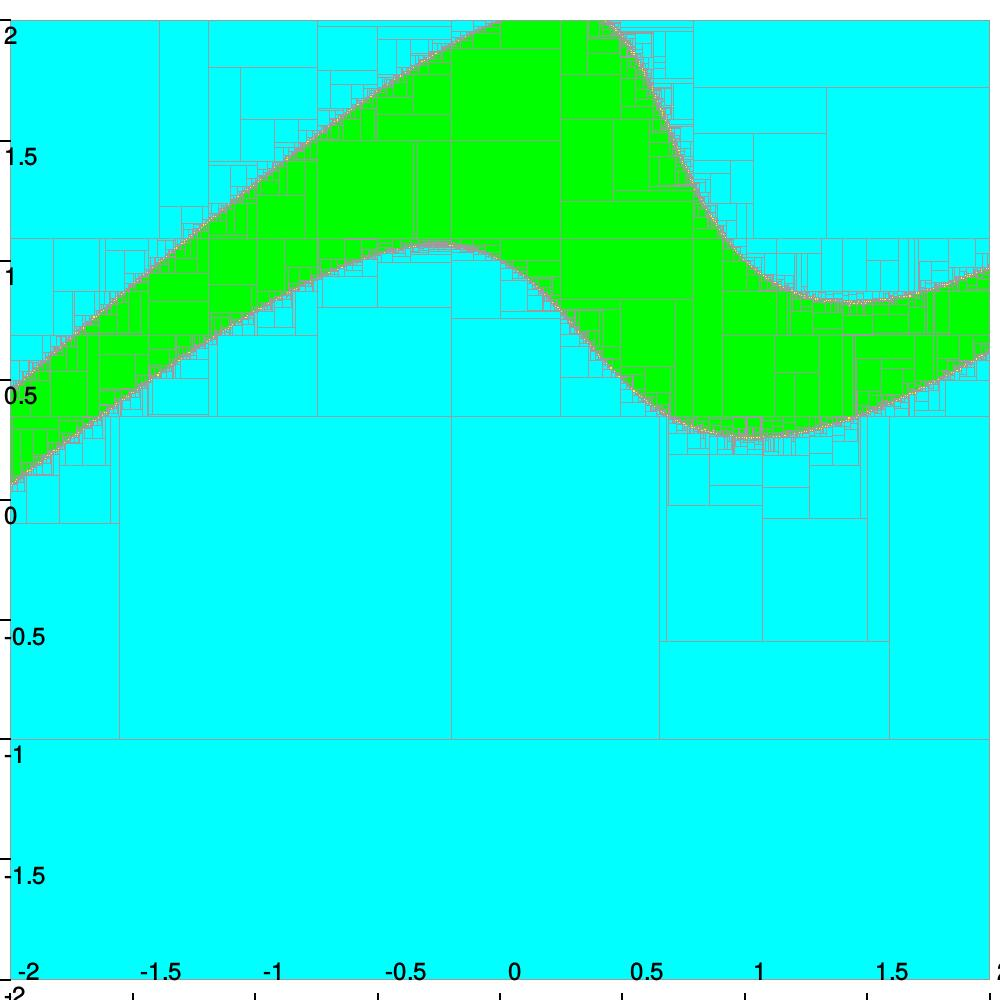
\includegraphics[width=.9\linewidth]{helloIntervals.jpg}
\end{center}
\end{document}